\documentclass[8pt]{beamer}

\usepackage{amsfonts}
\usepackage{subfiles}
\usepackage[T2A]{fontenc}
\usepackage[utf8]{inputenc}
\usepackage[russian]{babel}

\usepackage{amsmath, amsfonts, amssymb, amsthm, mathtools, mathrsfs}
\usepackage{wasysym, dsfont}
\usepackage{graphicx}
\usepackage{float}
\usepackage{wrapfig}

\usepackage{caption}
\usepackage{subcaption}
% \usepackage{subfigure}

\usepackage{multicol}

\mode<presentation>
{
	\usetheme{boxes}
	\beamertemplatenavigationsymbolsempty
	
	\setbeamertemplate{footline}[page number]
	\setbeamersize{text margin left=1.5em, text margin right=2.5em}
}


\title[]{Ускорение семплирования из диффузионных моделей с использованием состязательных сетей}
\author{Охотников Н.В}
\institute{МФТИ}
\date{2023}


\begin{document}

\begin{frame}
  \titlepage
\end{frame}


\begin{frame}
	\frametitle{Неявное моделирование обратного диффузионного процесса}



\end{frame}




	\setlength{\footskip}{1.8cm}
\begin{frame}
	\frametitle{Неявное моделирование обратного диффузионного процесса}


	\begin{columns}
		\begin{column}{0.5\textwidth}
			\begin{block}{Диффузионный процесс}
				\begin{itemize}
				
					\item Прямой: 
					\begin{equation*}
					q(\textbf{x}_t|\textbf{x}_{t-1}) = \mathcal{N}(\textbf{x}_t; \textbf{x}_{t-1}\sqrt{1-\beta_t}, \beta_t 	\textbf{I})
					\end{equation*}
					где $t = \overline{0,T}$, $\textbf{x}_0$ -- семпл из исходного распределения, $\textbf{x}_t$ -- семпл на шаге $t$, $\beta_t\in (0,1)$\\
					
					\item Обратный: 
					\begin{equation*}
					p_\theta(\textbf{x}_{t-1}|\textbf{x}_t)\!\! \underset{\text{T} \gg 1}{ \approx}\!\!\! \mathcal{N}(\textbf{x}_{t-1};\mu_\theta(\textbf{x}_t,t), \Sigma_\theta(\textbf{x}_t, t))
					\end{equation*}
			
				\end{itemize}
			\end{block}		
		\end{column}
		
		\begin{column}{0.55\textwidth} 
			
				\begin{figure}[h!]
						\begin{flushright}
							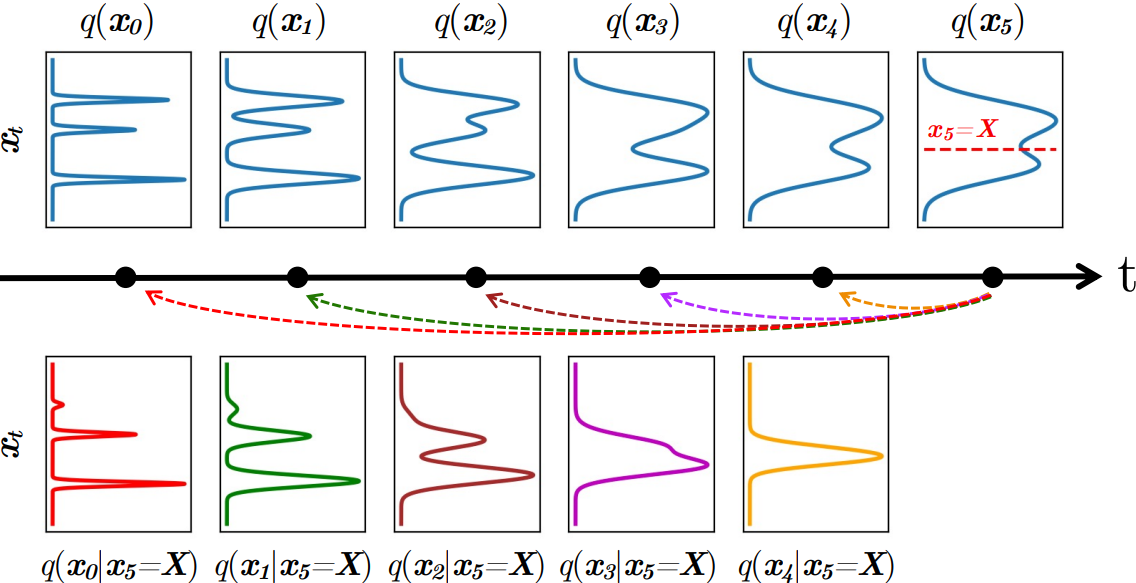
\includegraphics[width=0.97\textwidth]{figures/distributions.png}
						\end{flushright}		
				\end{figure}
	
		\end{column}
	\end{columns}


\begin{columns}
	\begin{column}{0.4\textwidth}
		
		\begin{block}{Основные предположения}
			
			\begin{itemize}	
				\item Марковость обратного процесса
				\item Нормальность и следовательно унимодальность $p_\theta(\textbf{x}_{t-1}|\textbf{x}_t)$
			\end{itemize}
		
		\end{block}
	
	\end{column}
	
	\begin{column}{0.57\textwidth}  
			\begin{block}{Предложение}
				\begin{itemize}
					\item Использовать неявную модель для восстановления распределения
				\end{itemize}
			\end{block}	
		\begin{block}{Мотивация}
			\begin{itemize}
				\item Моделирование мультимодального распределения для существенного уменьшения T
			\end{itemize}
		\end{block}	
	\end{column}
\end{columns}
\small{\url{https://doi.org/10.48550/arxiv.2112.07804}}
\end{frame}
\end{document}



\end{document}
